\begin{filecontents*}{presentation.bib}
@article{Kaelin:2005gm,
	author = {Kaelin, William G},
	title = {{The concept of synthetic lethality in the context of anticancer therapy.}},
	journal = {Nat. Rev. Cancer},
	year = {2005}
}
@article{thanei2018xyz,
	title={The xyz algorithm for fast interaction search in high-dimensional data},
	author={Thanei, Gian-Andrea and Meinshausen, Nicolai and Shah, Rajen D},
	journal={The Journal of Machine Learning Research},
	volume={19},
	number={1},
	pages={1343--1384},
	year={2018},
	publisher={JMLR. org}
}
\end{filecontents*}

\documentclass[8pt]{beamer}
\usetheme{Hannover}

\usepackage[style=numeric,firstinits=true,backend=biber]{biblatex}
\addbibresource{presentation.bib}
\usepackage{todonotes}

\presetkeys{todonotes}{inline}{}

%\geometry{paperwidth=140mm,paperheight=105mm}

\title{Inferring Genetic Interactions: Comparing \texttt{xyz} and \texttt{glinternet}}
\author{Kieran Elmes}
\begin{document}
\begin{frame}[plain]
    \maketitle
\end{frame}

\section{Background}
\begin{frame}{The Problem}
\begin{minipage}{0.4\linewidth}
	\includegraphics[width=0.8\linewidth]{"cells_2x"}\\[-1ex]
	{\tiny Obligatory xkcd\\Source: \href{https://www.xkcd.com/1217/}{https://www.xkcd.com/1217/}}
\end{minipage}%
\begin{minipage}{0.6\linewidth}
	\begin{itemize}
		\item Killing cancer cells is easy. Killing cancer cells selectively is hard.
		\item Synthetic lethal interactions could potentially be used for exactly that.\cite{Kaelin:2005gm}
		\item We have approx. 20,000 genes. Experimentally testing all 200 million pairwise interactions is awkward.
	\end{itemize}
\end{minipage}
\end{frame}

\begin{frame}{What are we doing}
\begin{itemize}
	\item Simulating large(ish) sets of SiRNA knockdowns, and measuring xyz's ability to correctly determine interactions in the data.
	\item We can already do this with glinternet, but \texttt{xyz} is (several hundred times?) faster.
	\item \texttt{xyz} $= O(p^\alpha)$ for $1 < \alpha < 2$, depending on the strength of the interactions.
\end{itemize}
\end{frame}

\begin{frame}{The Data}
\begin{itemize}
	\item SiRNAs can reduce the expression of several hundred genes at once.
	\item $X \leftarrow n \times p$ matrix, $n$ trials with $p$ affected genes.
	\item $Y \leftarrow p$ fitness values.
\end{itemize}
\end{frame}

%\begin{center}
%\includegraphics[width=\textwidth]{../interactions-perf-manuscript/figures/Figure_Pmat.pdf}
%\includegraphics[width=0.9\textwidth]{figures/Figure_PRFinteractions.pdf}

\begin{frame}{Runtime comparison}
\centering
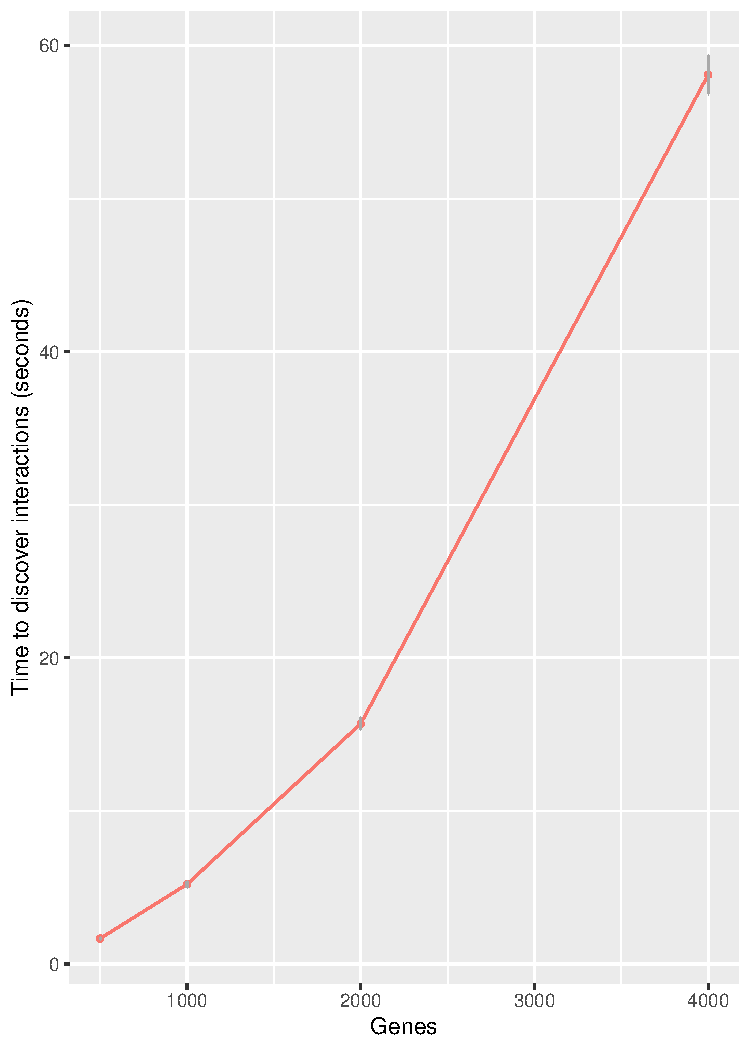
\includegraphics[width=0.45\linewidth]{time_taken/time_taken_xyzTRUE}%
\includegraphics[width=0.45\linewidth]{time_taken/time_taken_xyzFalse}

\hspace{2.8cm} \texttt{xyz} \hfill \texttt{glinternet} \hspace{1.8cm}
\end{frame}

\begin{frame}{\texttt{glinternet}: $p = 100$}
\includegraphics[width=0.5\linewidth]{output/PrecRecF1_n1000_tno_large0_xyzFalse_}%
\includegraphics[width=0.5\linewidth]{output/PrecRecF1_n1000_tyes_large0_xyzFalse_}
\end{frame}

\begin{frame}
\centering
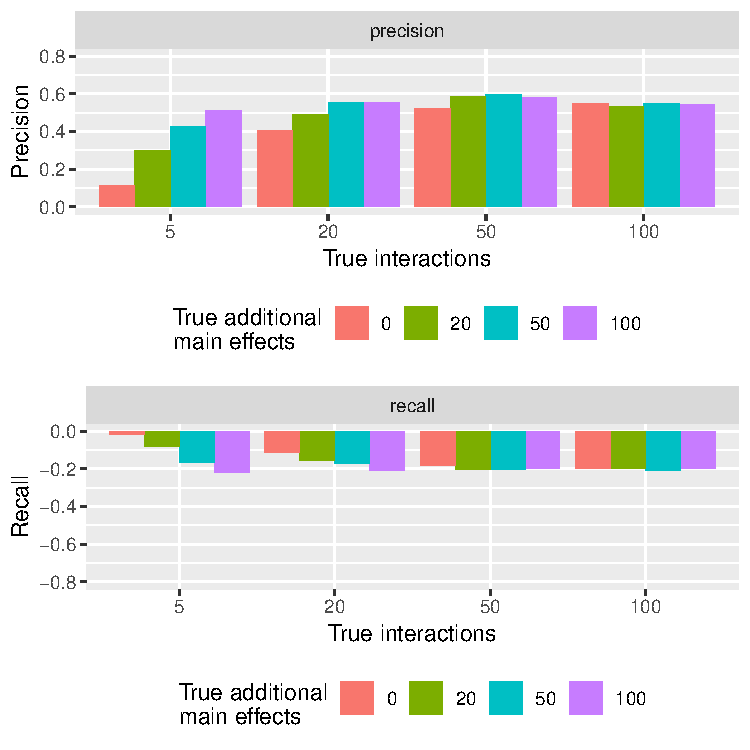
\includegraphics[width=0.6\linewidth]{output/test_analysis_n1000_large0_xyzFALSE_}
\end{frame}

\begin{frame}{\texttt{xyz}: $p = 100$}
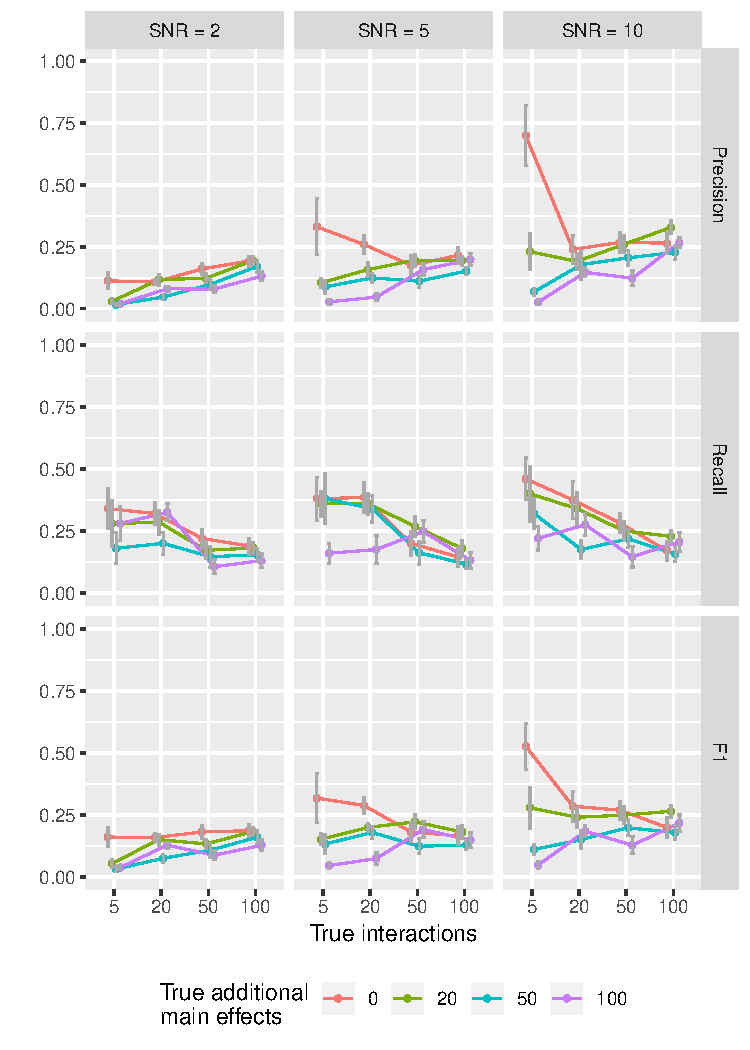
\includegraphics[width=0.5\linewidth]{output/PrecRecF1_n1000_tno_large0_xyzTRUE_}%
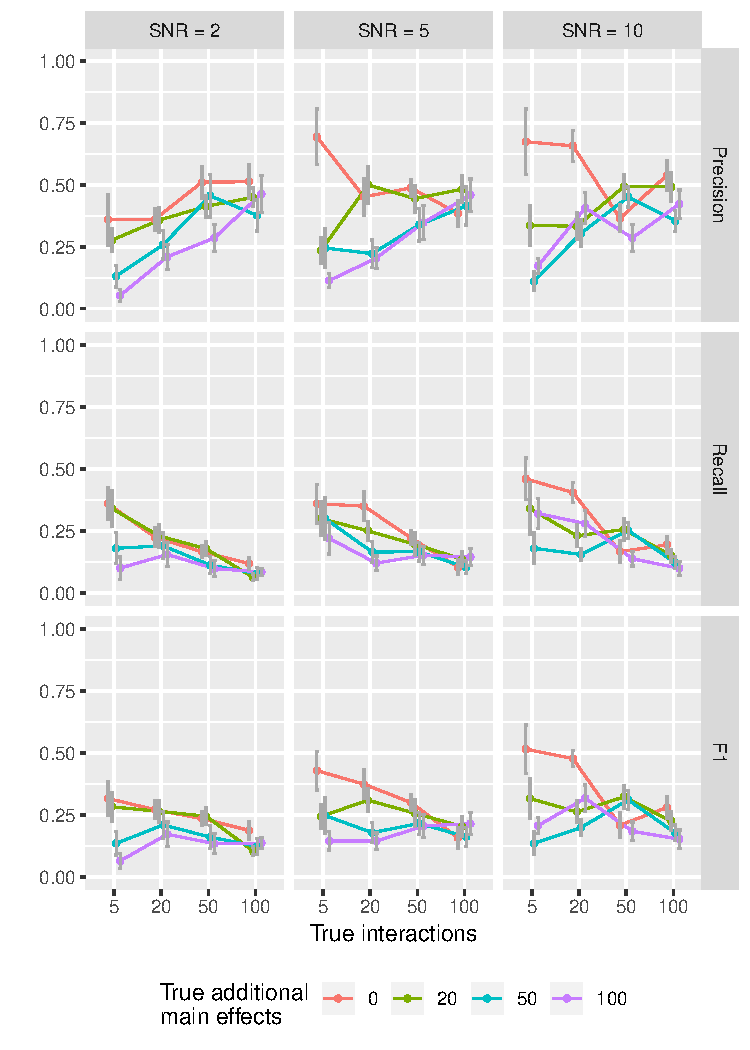
\includegraphics[width=0.5\linewidth]{output/PrecRecF1_n1000_tyes_large0_xyzTRUE_}
\end{frame}

\begin{frame}
\centering
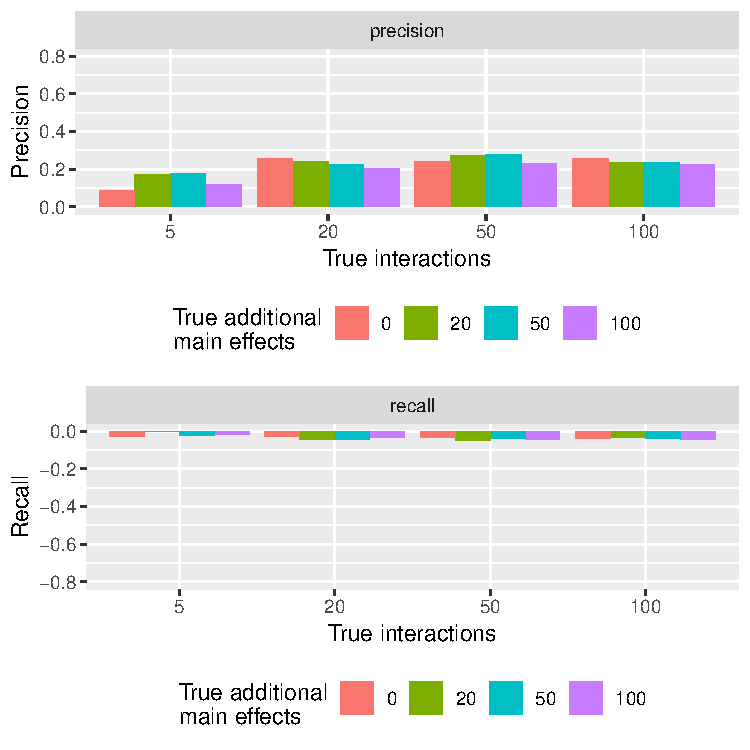
\includegraphics[width=0.6\linewidth]{output/test_analysis_n1000_large0_xyzTRUE_}
\end{frame}

\begin{frame}{\texttt{xyz}: $p = 1000$}
\includegraphics[width=0.5\linewidth]{output/PrecRecF1_n10000_tno_large1_xyzTRUE_}%
\includegraphics[width=0.5\linewidth]{output/PrecRecF1_n10000_tyes_large1_xyzTRUE_}
\end{frame}

\begin{frame}
\centering
\includegraphics[width=0.6\linewidth]{PrecRecF1/test_analysis_n10000_large1_xyzTRUE_}
\end{frame}


%\includegraphics[width=\textwidth]{figures/Figure_PRFobservations.pdf}
%\begin{frame}
%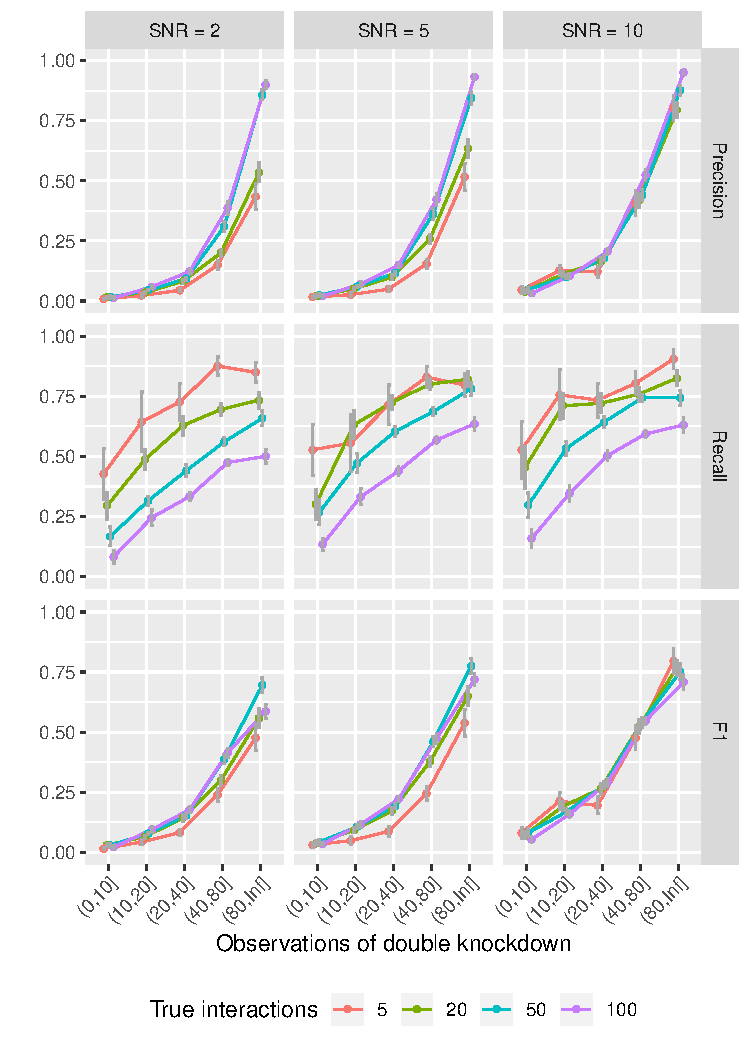
\includegraphics[width=0.5\linewidth]{output/NumObservations_n1000_tno_xyzFALSE}%
%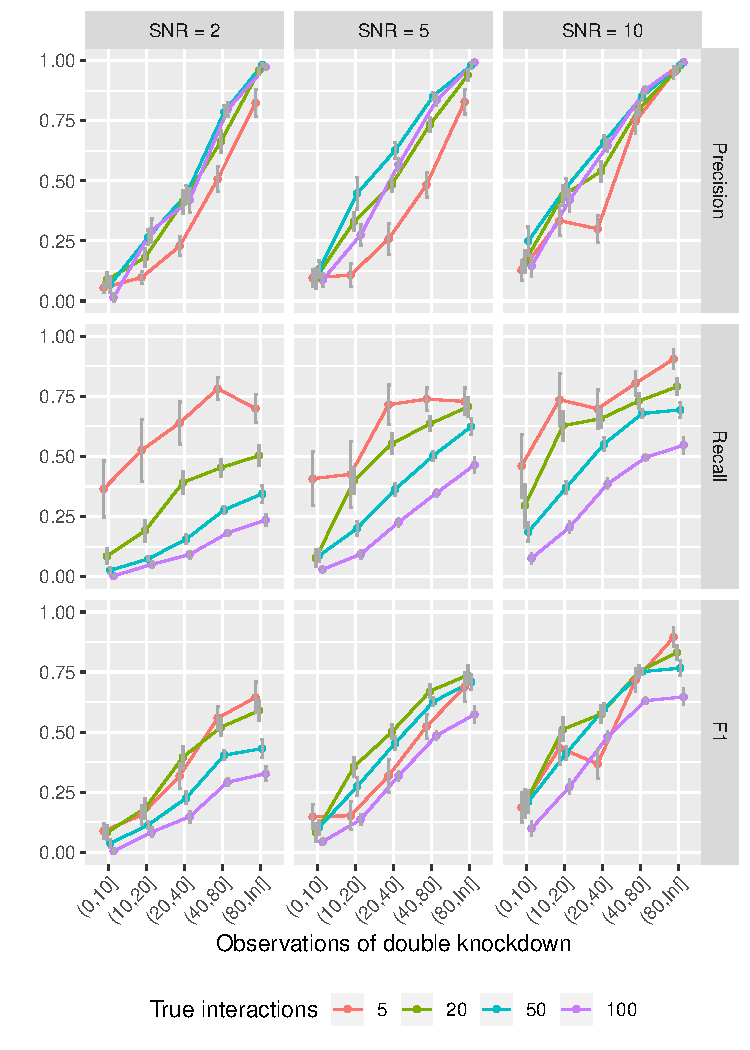
\includegraphics[width=0.5\linewidth]{output/NumObservations_n1000_tyes_xyzFALSE}
%\end{frame}

\section{\texttt{xyz} performance}

\begin{frame}{\texttt{xyz}: Number of observations of each pair}
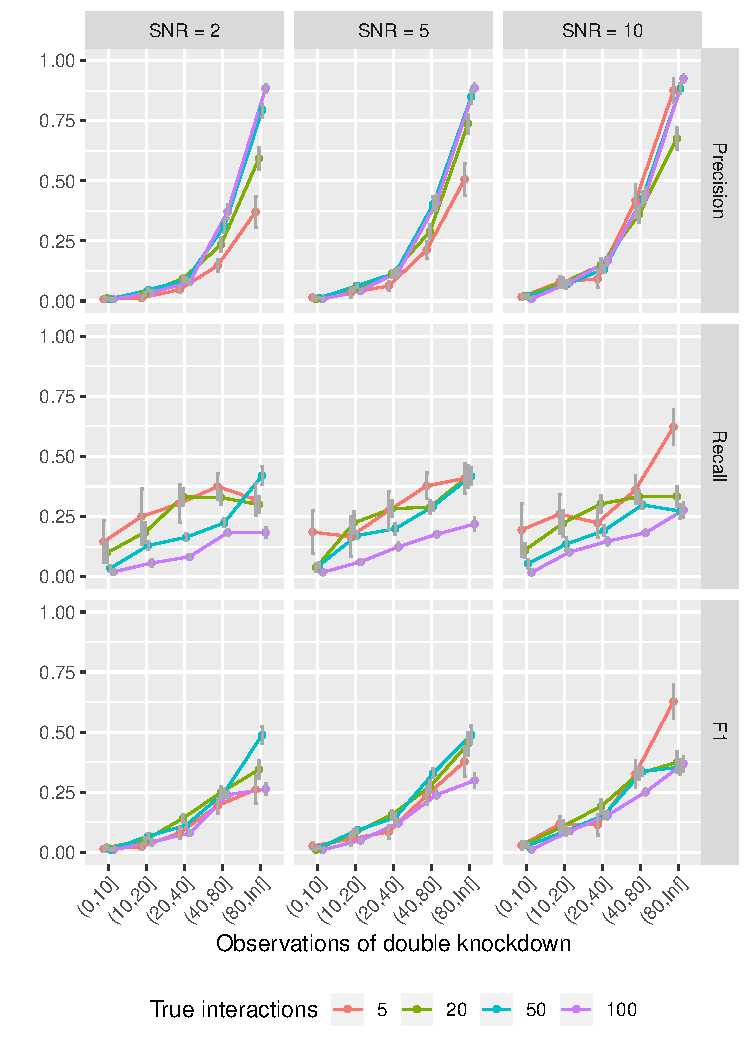
\includegraphics[width=0.5\linewidth]{output/NumObservations_n1000_tno_xyzTRUE}%
\includegraphics[width=0.5\linewidth]{output/NumObservations_n10000_tno_xyzTRUE}%
\end{frame}


\begin{frame}
\includegraphics[width=0.5\linewidth]{"../interactions-perf-manuscript/output/NumObservations_n1000_percGenes"}%
\includegraphics[width=0.5\linewidth]{"../interactions-perf-manuscript/output/NumObservations_n10000_percGenes"}
\end{frame}

\begin{frame}{\texttt{xyz}: Effect strength}
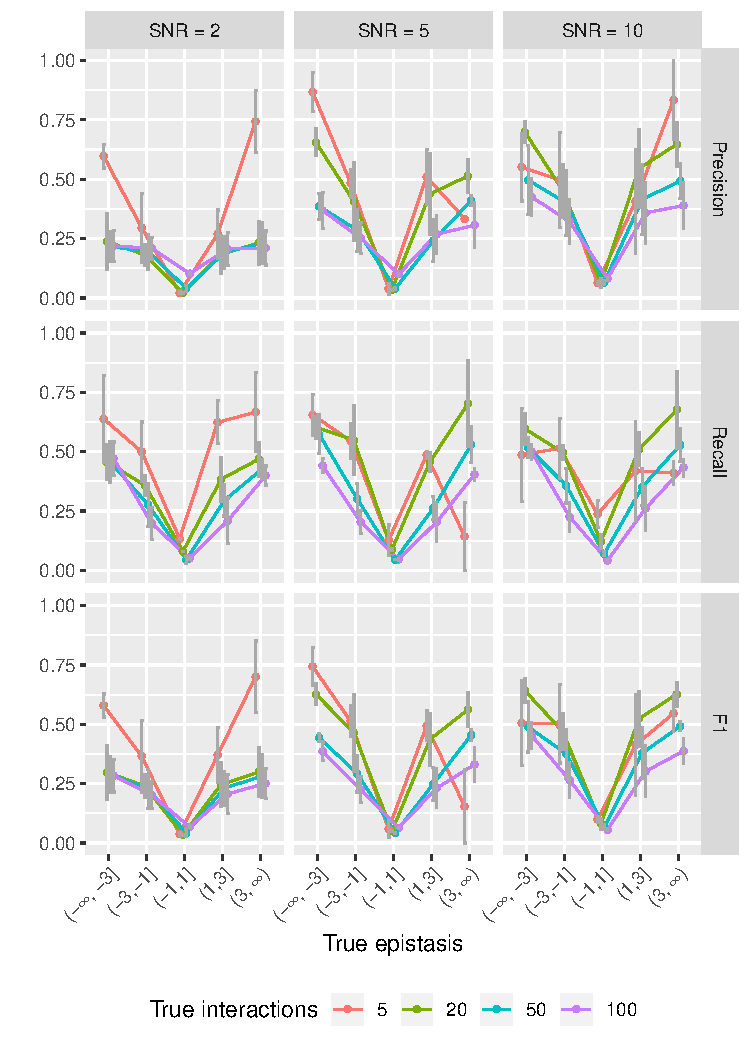
\includegraphics[width=0.5\linewidth]{output/FXstrength_PRF_n1000_tno_mult1_xyzTRUE_}%
\includegraphics[width=0.5\linewidth]{output/FXstrength_PRF_n10000_tno_mult10_xyzTRUE_}
\end{frame}

%\begin{frame}{Effect direction}
%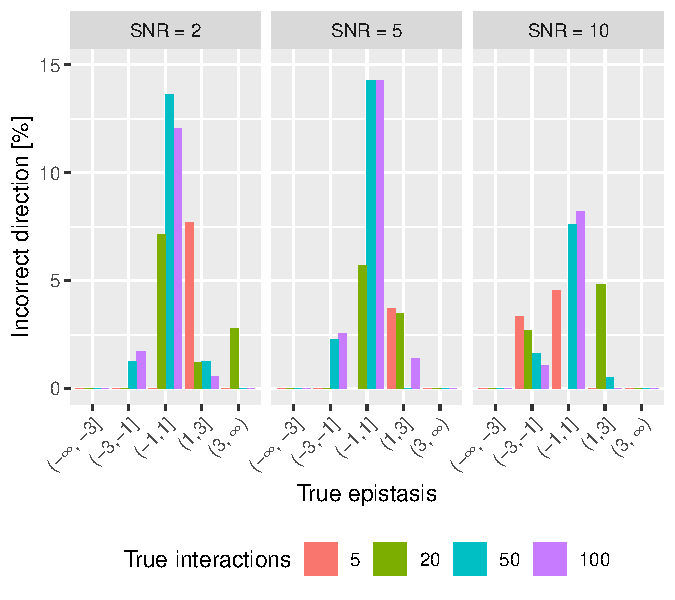
\includegraphics[width=0.5\linewidth]{output/FXstrength_direction_n1000_tno_mult1_xyzTRUE_}%
%\includegraphics[width=0.5\linewidth]{output/FXstrength_direction_n10000_tno_mult10_xyzTRUE_}
%\end{frame}

%\begin{frame}
%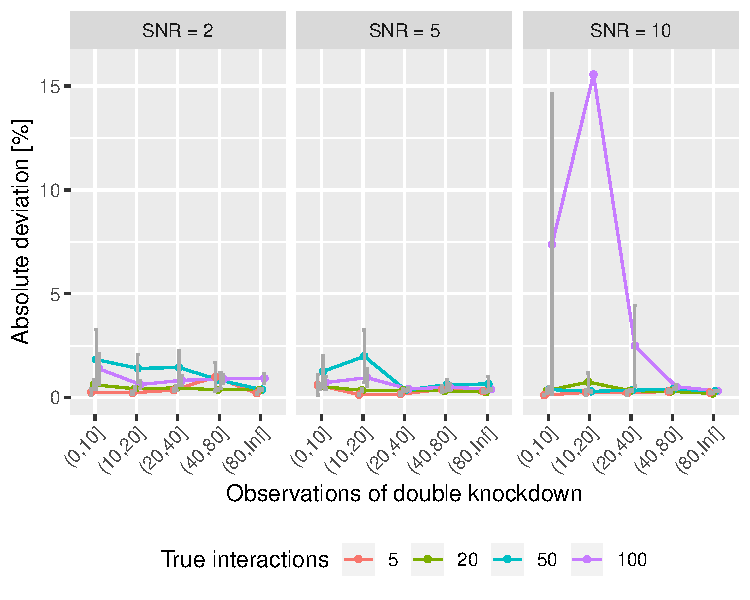
\includegraphics[width=0.5\linewidth]{output/FXdiff_n1000_tno_xyzTRUE}%
%\includegraphics[width=0.5\linewidth]{output/FXdiff_n10000_tno_xyzTRUE}
%\end{frame}

%\begin{frame}
%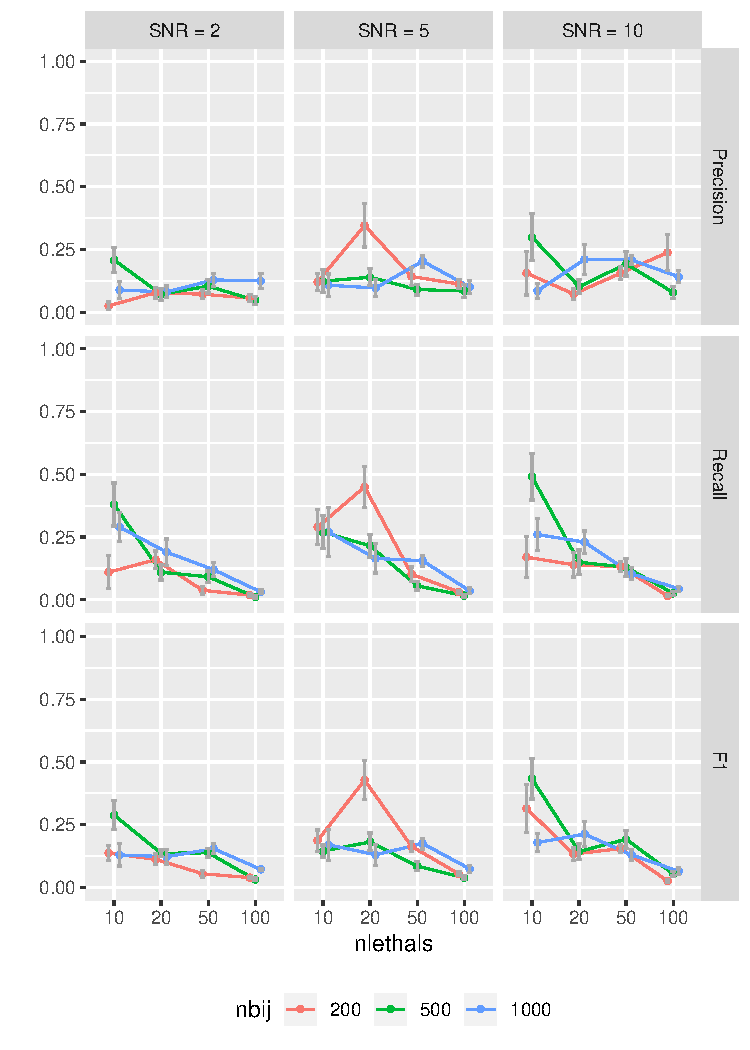
\includegraphics[width=0.5\linewidth]{output/PrecRecF1_n10000_tno_large0_lethalTRUE_lethal}%
%\includegraphics[width=0.5\linewidth]{small_xyz_50times/large_lethal_n5000_tno_large0_xyzTRUE_lethal}
%\end{frame}

\begin{frame}{Scalability: xyz}
\includegraphics[width=0.5\linewidth]{../interactions-perf-manuscript/output/large_lethal_n5000_tno_large0_xyzTRUE_lethal}%
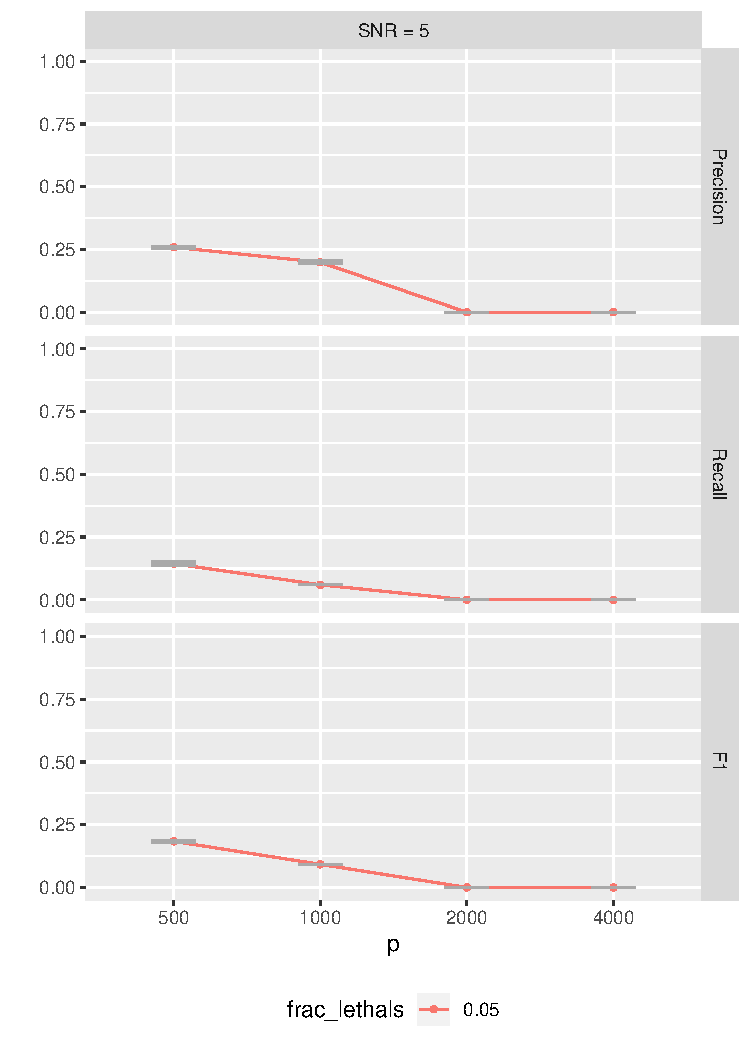
\includegraphics[width=0.5\linewidth]{../interactions-perf-manuscript/output/large_lethal_n5000_tyes_large0_xyzTRUE_lethal}
\end{frame}

\section{Scalability}
\begin{frame}{Scalability: glinternet}
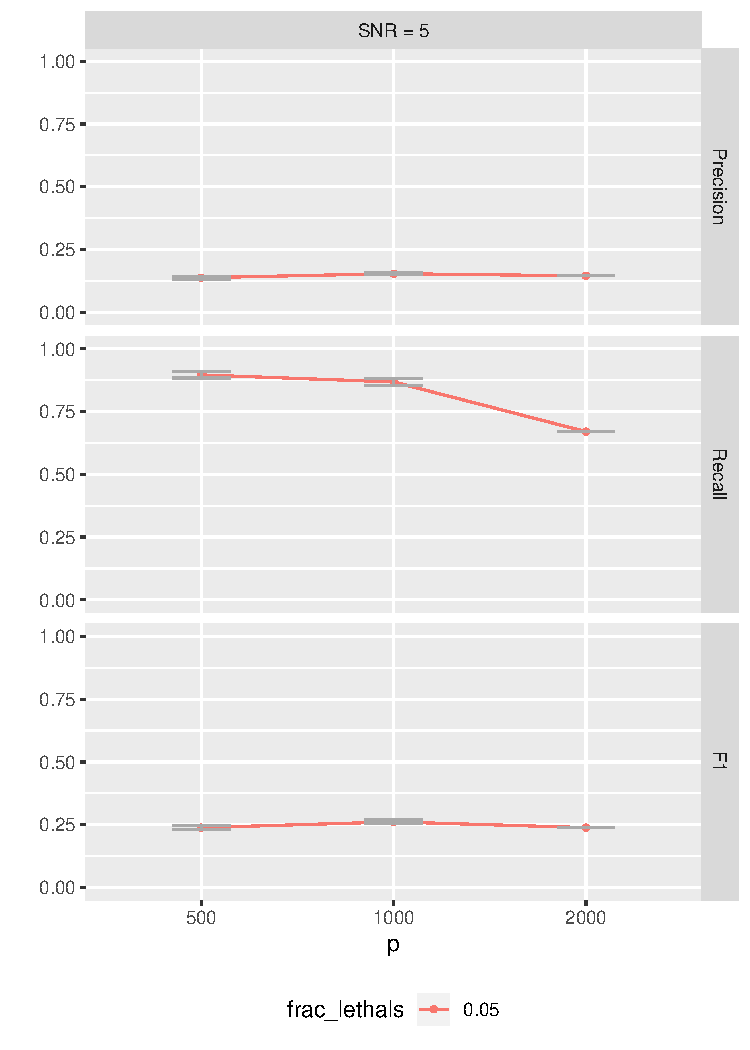
\includegraphics[width=0.5\linewidth]{../interactions-perf-manuscript/output/large_lethal_n5000_tno_large0_xyzFALSE_lethal}%
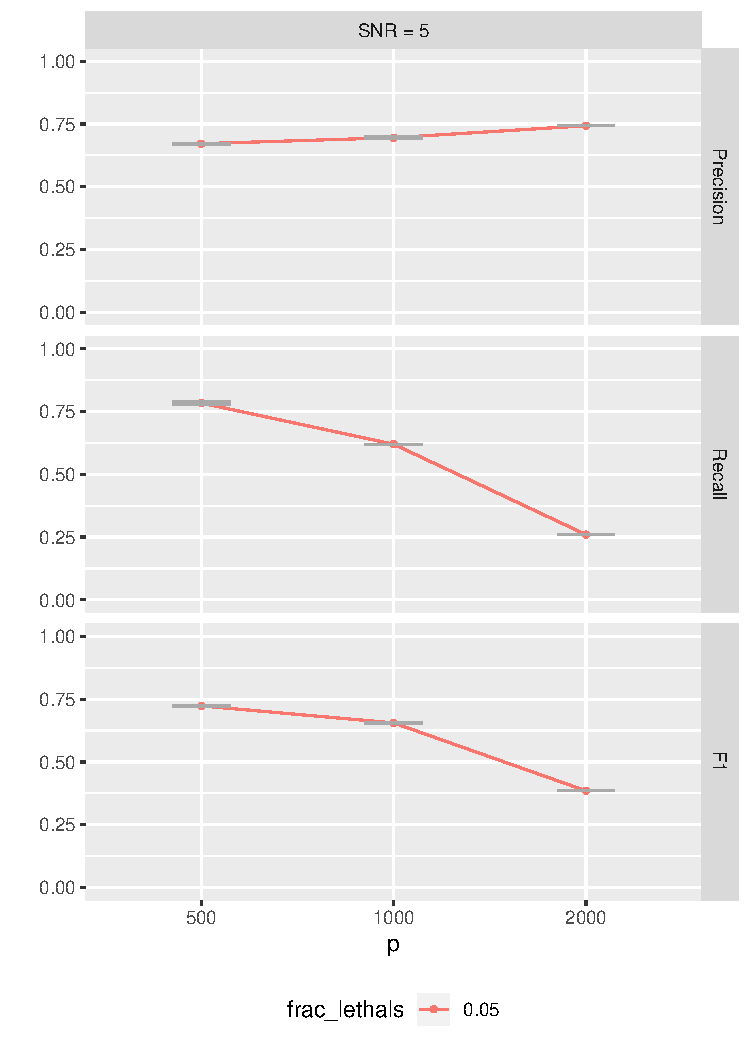
\includegraphics[width=0.5\linewidth]{../interactions-perf-manuscript/output/large_lethal_n5000_tyes_large0_xyzFALSE_lethal}
\end{frame}

\section{glinternet performance}

\begin{frame}{\texttt{glinternet}: Number of observations of each pair}
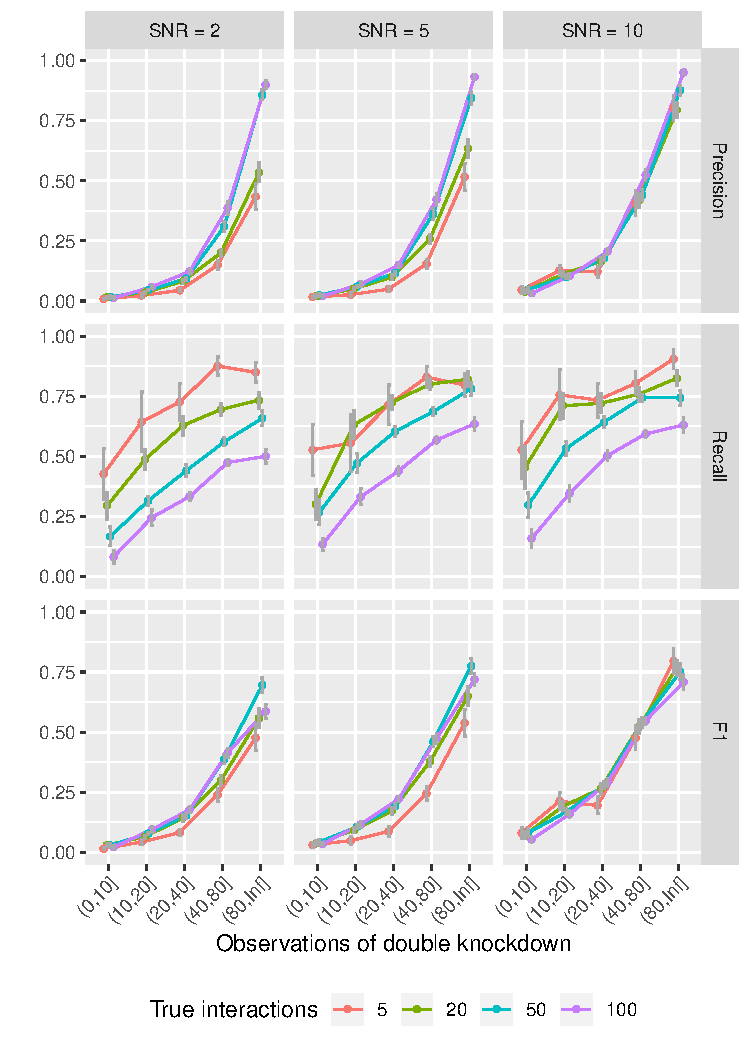
\includegraphics[width=0.5\linewidth]{output/NumObservations_n1000_tno_xyzFALSE}%
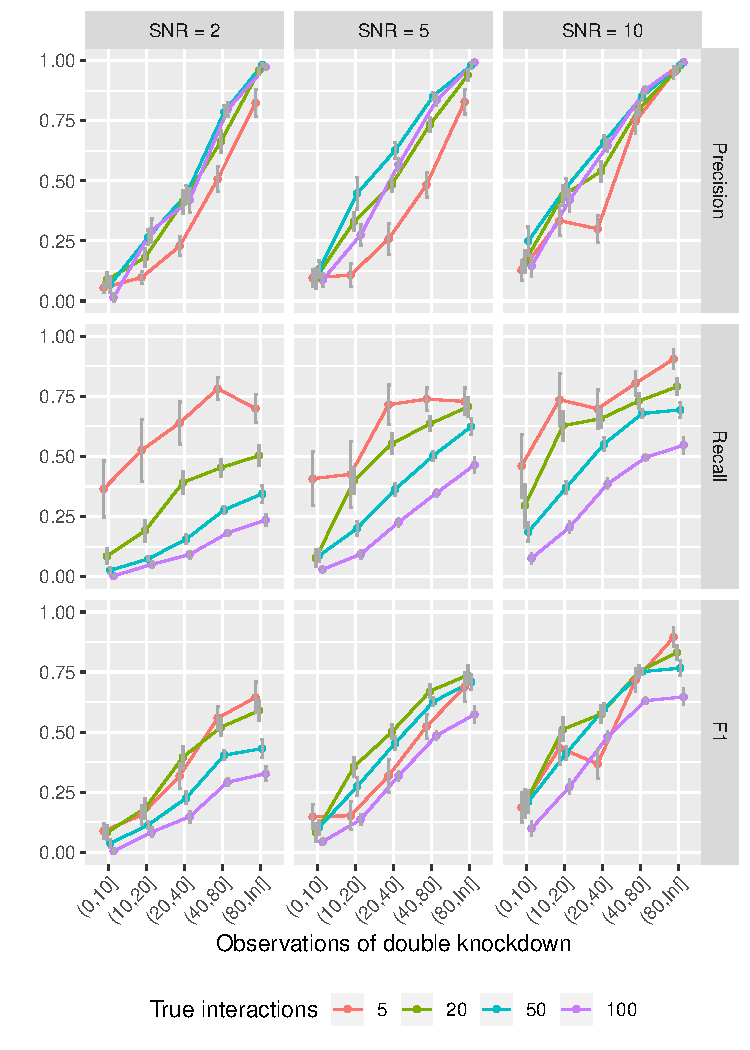
\includegraphics[width=0.5\linewidth]{output/NumObservations_n1000_tyes_xyzFALSE}%
\end{frame}

\begin{frame}{\texttt{glinternet}: Effect strength}
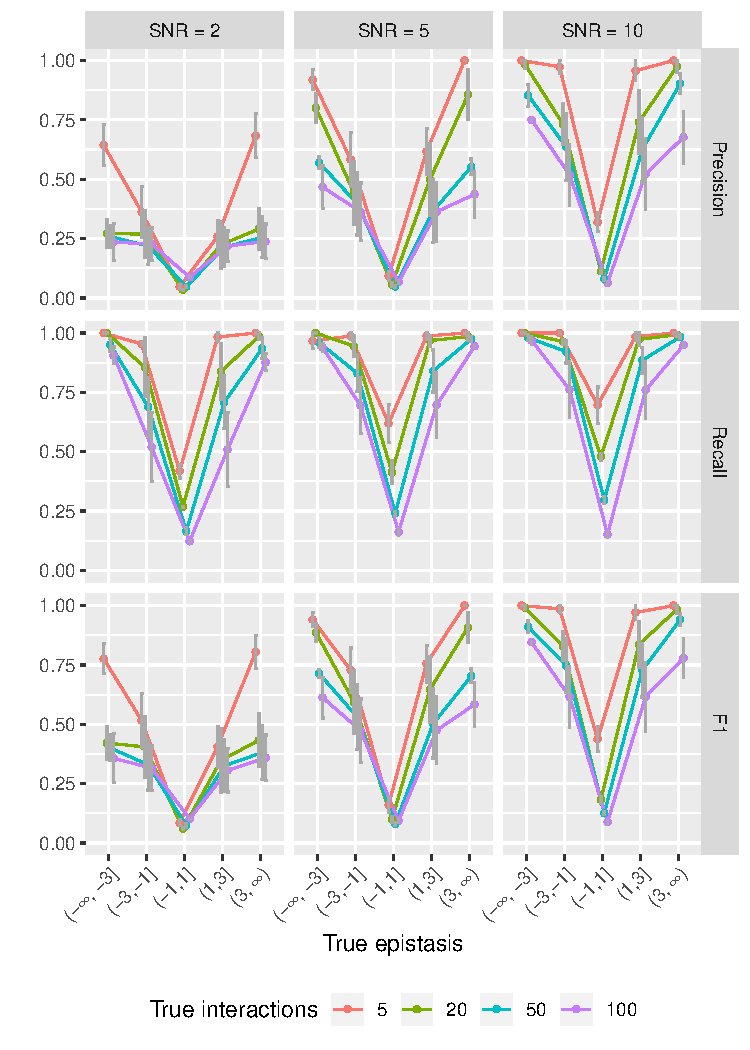
\includegraphics[width=0.5\linewidth]{output/FXstrength_PRF_n1000_tno_mult1_xyzFALSE_}%
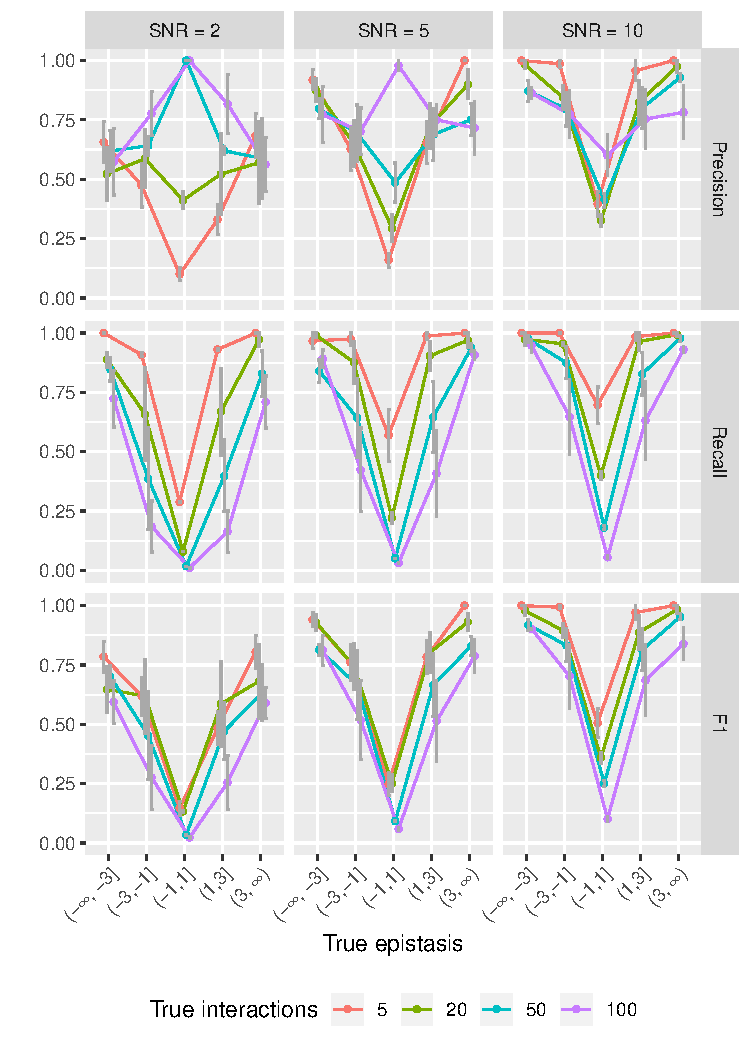
\includegraphics[width=0.5\linewidth]{output/FXstrength_PRF_n1000_tyes_mult1_xyzFALSE_}
\end{frame}

\begin{frame}{\texttt{glinternet}: Effect direction}
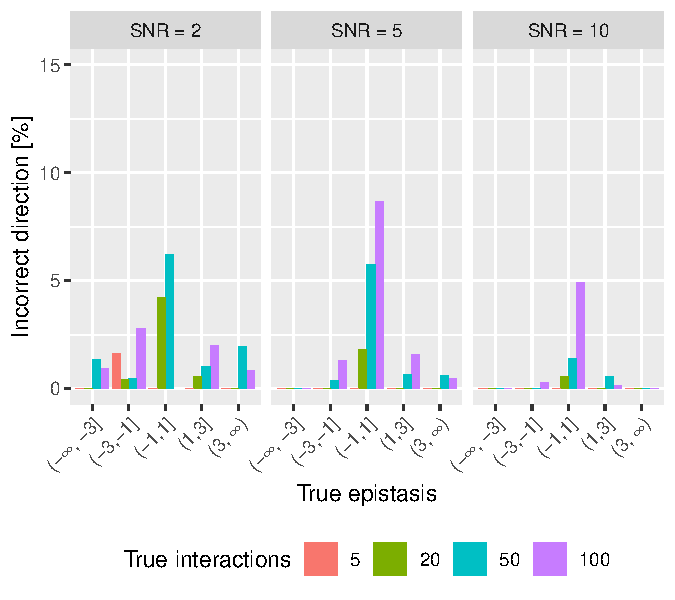
\includegraphics[width=0.5\linewidth]{output/FXstrength_direction_n1000_tno_mult1_xyzFALSE_}%
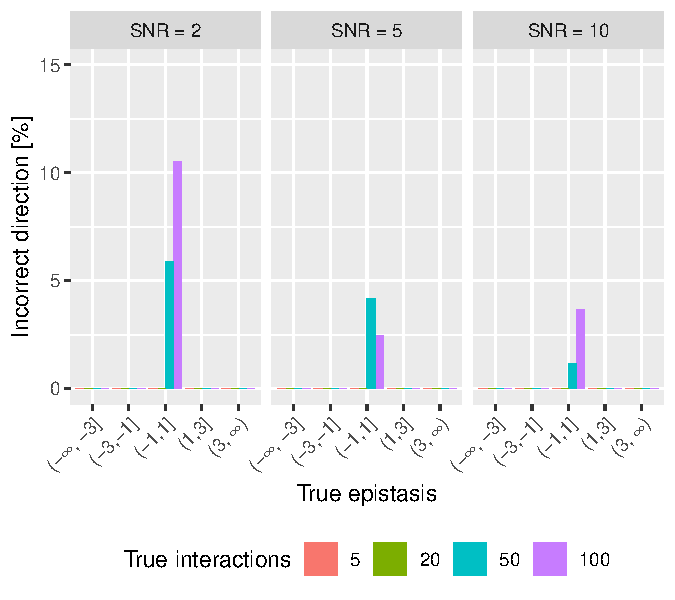
\includegraphics[width=0.5\linewidth]{output/FXstrength_direction_n1000_tyes_mult1_xyzFALSE_}
\end{frame}

\begin{frame}
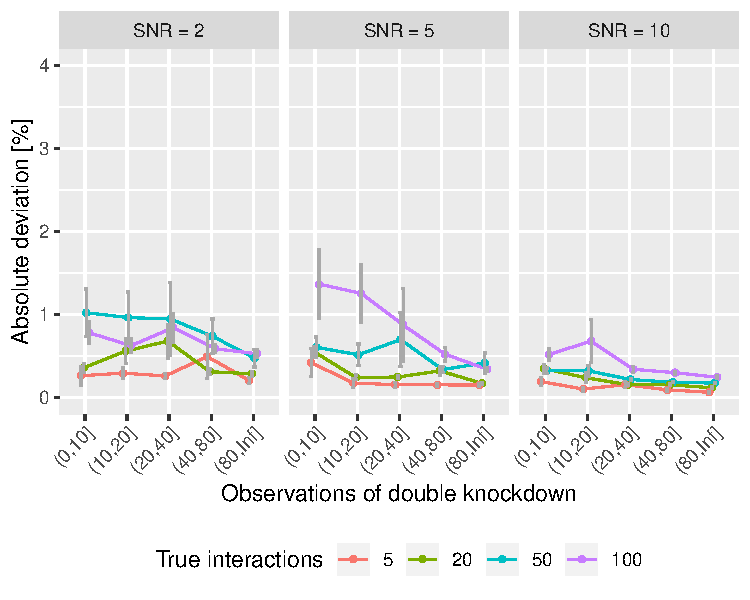
\includegraphics[width=0.5\linewidth]{output/FXdiff_n1000_tno_xyzFALSE}%
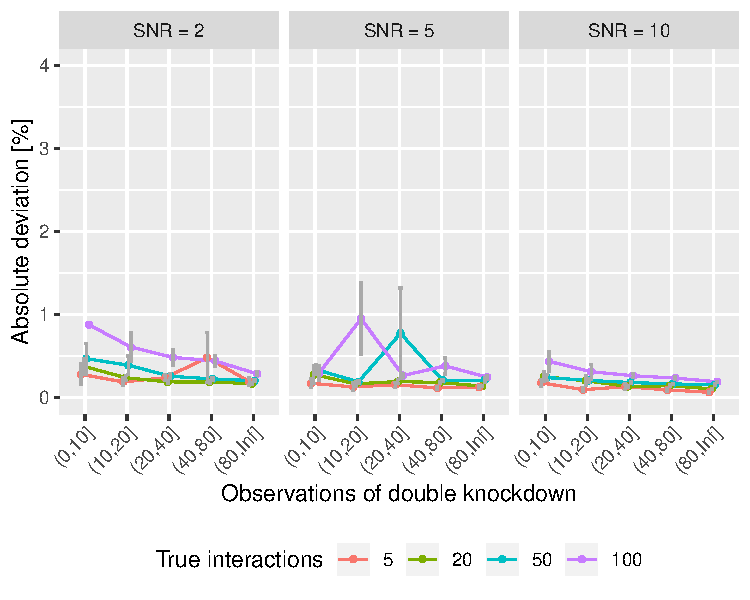
\includegraphics[width=0.5\linewidth]{output/FXdiff_n1000_tyes_xyzFALSE}
\end{frame}

\section{Parameter choices \& model Assumptions}
\begin{frame}{Choice of $L$}
\centering
\includegraphics[width=0.45\linewidth]{"../interactions-perf-manuscript/output/l_diff_n10000_SNR5_tno"}%
\includegraphics[width=0.45\linewidth]{"output/quant_analysis_n10000"}
\end{frame}

\begin{frame}{Distribution of \texttt{xyz} failures}
\centering
\includegraphics[width=0.5\linewidth]{../interactions-perf-manuscript/failed_xyz_distribution}
\end{frame}

\begin{frame}{Summary}
\begin{enumerate}
	\item \texttt{xyz} works for data small enough that we don't need it.
	\item \texttt{glinternet} (probably) works for data too large to practically use it.
\end{enumerate}
\end{frame}

%\end{center}
\end{document}



% Things to mention: (also see notes)
